\section{Introduction}
Embedding models play a crucial role in connecting data across various modalities. By encoding heterogeneous multimodal data into a shared dense representation space, they enable many down-stream applications like classification, clustering, retrieval. In recent years, we have witnessed significant advances in embedding models, largely driven by the progress of large foundation models. For instance, recent breakthroughs in text embedding \citep{instructor,e5mistral, SFRembedding,LLM2Vec} have been achieved by integrating pretrained large language models with multi-task instruction embedding tuning. Similarly, \citet{vlm2vec,gme, chen-etal-2025-seeing} demonstrated strong performance across multiple text-image tasks by instruction-tuning multimodal large language models (MLLMs) into effective embedding models.


Existing multimodal embedding models are trained on datasets like MMEB~\citep{vlm2vec} and M-BEIR~\citep{uniir}, which are focused predominantly on natural images or photographs, sourced from MSCOCO~\citep{mscoco}, Flickr~\citep{flickr30k} and ImageNet~\citep{imagenet} datasets. These datasets fail to cover broader forms of visual information, such as documents, PDFs, websites, and videos. 

This limited coverage makes existing embedding models overly domain-specific and prevents them from generalizing well to realistic tasks such as document retrieval and YouTube video search. We empirically validate this claim in our experiments (Table \ref{tab:main_exp}). A model trained exclusively on visual documents, such as Colpali~\citep{colpali}, achieves strong performance on document tasks (71.0\%) but suffers a severe performance drop on image (34.9\%) and video tasks (28.2\%). Conversely, a model trained solely on image data, such as \vlmvec (2B)~\citep{vlm2vec}, excels on image tasks (59.7\%) but performs substantially worse on document (41.6\%) and video tasks (29.0\%).

%The limited coverage of video-based tasks and visual documents in existing benchmarks restricts our ability to evaluate the generalization capability of embedding models across diverse modalities and real-world scenarios. 
%Key challenges such as temporal grounding within videos~\citep{qvhighlights,momentseeker} or retrieving information from multi-page documents like PDFs~\cite{colpali,mmlongbench} and presentation slides~\citep{slidevqa} are largely underrepresented in current evaluation frameworks. 

% \begin{figure}[!t]
%     \centering
%     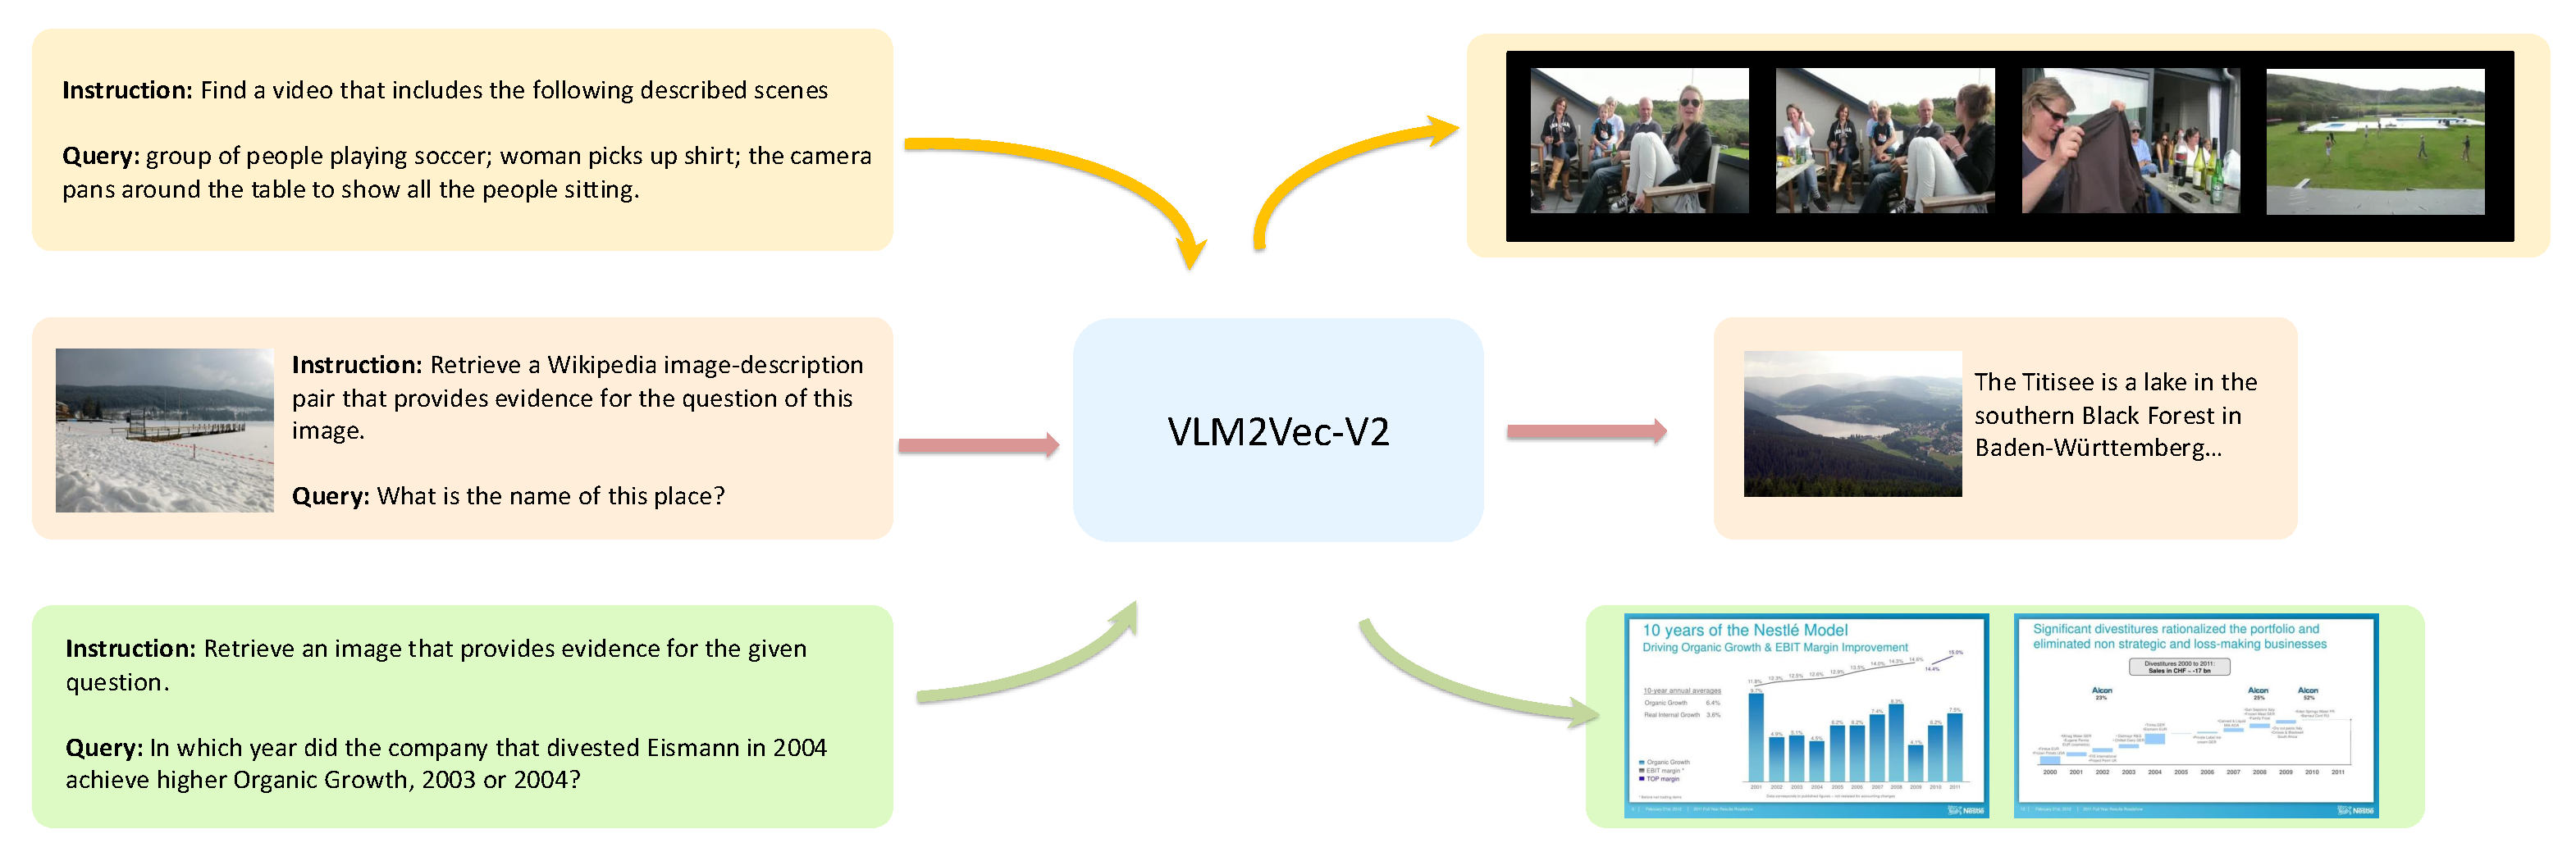
\includegraphics[width=\linewidth]{figures/teaser.pdf}
%     \caption{\model unifies embedding learning across videos, images, and visual documents.}
%     \label{fig:teaser}
%     \vspace{-3pt}
% \end{figure}

To address these limitations, we introduce \benchmark, an advanced multimodal embedding dataset designed to train and evaluate embedding models across three key visual modalities: images, videos, and visual documents. Expanding on the original \mmeb~\citep{vlm2vec} framework, \benchmark broadens the evaluation scope to encompass five new tasks, including four video-based tasks—Video Retrieval, Moment Retrieval, Video Classification, and Video Question Answering — as well as one task centered on visual documents: Visual Document Retrieval. This comprehensive suite of tasks allows for robust assessment of multimodal embedding models across static, temporal, and structured visual data settings.

Built on top of \benchmark, we propose \textbf{\model}, a framework that adapts state-of-the-art multimodal large language models, such as Qwen2-VL~\citep{qwen2vl}, into a unified embedding model. \model is trained using a mixture of instruction-following tasks spanning multiple task categories, enabling it to learn unified representations across a wide range of visual modalities.

In this paper, we adopt Qwen2-VL-2B as the base model for all experiments, balancing computational cost with the inclusion of video training data. Our framework is general and can be readily scaled to larger MLLMs.




% Through \model and \benchmark, we aim to investigate the following research question: How well can a multimodal embedding generalize across diverse visual modalities? 
% What are the key ingredients for training robust and versatile multimodal embedding models?

% \textcolor{red}{Give some highlights about the results. @Rui}

The contributions of this work are threefold.
\begin{itemize}[
    itemsep=0pt,        % remove space between items
    parsep=0pt,         % remove paragraph spacing within items
    topsep=0pt,         % remove extra space at the top
    leftmargin=1em      % adjust the left margin as needed
]
\item We propose \benchmark, a comprehensive dataset for systematically evaluating embedding models on diverse tasks involving videos, images, and visual documents.
\item We develop \model, a unified multimodal embedding framework that supports instruction following to produce general-purpose embeddings for a wide range of downstream tasks.
\item Our experiments demonstrate that the 2B-parameter version of \model outperforms prior baselines across 78 datasets. Through detailed ablation studies, we identify effective training strategies for learning multimodal embedding models.
\end{itemize}

